

\section{Theoretical modeling of signal and background processes}
\label{mcgeneration}

In this section we discuss the settings of the
Monte Carlo generation of the signal and background
processes used in this analysis.
%
We also discuss the modelling of finite detector
resolution effects by means of an smearing of the final-state
particles four-momenta.

\subsection{Higgs pair production in gluon-fusion}


%%%%%%%%%%%%%%%%%%%%%%%%%%%%
\begin{figure}[t]
\begin{center}
  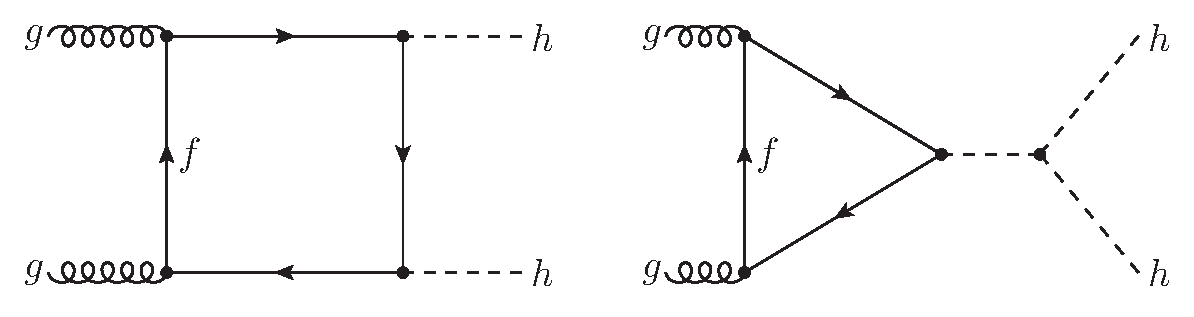
\includegraphics[width=0.90\textwidth]{plots/hhFeyn.pdf}
  \caption{\small Representative Feynman diagrams
    for Higgs pair production in gluon fusion at
    leading order.
    %
    Only the quark triangle diagram (left) is sensitive to the Higgs trilinear coupling
    $\lambda$.
    %
    In the SM, the fermion loops are dominated by the top quark contribution.
}
\label{fig:hhFeyn}
\end{center}
\end{figure}
%%%%%%%%%%%%%%%%%%%%%%%

Higgs pair production is simulated at leading order using
{\tt MadGraph5\_aMC@NLO}~\cite{Alwall:2014hca}.
%
We use a tailored {\tt MadGraph5\_aMC@NLO} model~\cite{Maltoni:2014eza} that simulates
gluon-gluon-fusion Higgs boson pair production including the effects
of the
exact form factors for the top triangle and box loops at leading
order, the latter taken from from~\cite{Plehn:1996wb}.\footnote{We note that since recently it is possible to compute also
loop-induced processes in {\tt MadGraph5\_aMC@NLO} without the need of using specific
models~\cite{Hirschi:2015iia}.}
%
We use the default settings of the renormalization and factorization
scale of the model.
%
The Higgs boson parameters are also the same in the default model,
in particular we use $m_h=125$ GeV, consistent with the latest
measurements from ATLAS and CMS~\cite{Aad:2014aba,Khachatryan:2014jba}.
%
The value of the Higgs trilinear coupling $\lambda$ is set to its
Standard Model value.
%
The calculation is performed in the
$n_f$=4 scheme and thus
takes into account the finite mass of the $b$-quarks.
%
For the input parton distribution functions, we 
adopt the NNPDF 3.0 $n_f = 4$ LO set~\cite{Ball:2014uwa} with
$\alpha_s(m_Z^2)=0.118$
interfaced via {\tt LHAPDF6}~\cite{Buckley:2014ana}.

In Fig.~\ref{fig:hhFeyn} we show representative Feynman diagrams
    for Higgs pair production in gluon fusion at
    leading order.
    %
    The non-trivial interplay between the diagram with a heavy quark box
    and that of the triangle, that can lead to constructive or destructive interference,
    complicates the extraction of
    the trilinear coupling
    $\lambda$ from the measurement of the Higgs pair
    production cross-section.
    %
    Higher order corrections are dominated by gluon radiation
    from either the initial state gluons or from the heavy quark loops.

    The total inclusive cross-section for this processes is
    known up to NNLO~\cite{deFlorian:2013jea}.
    %
Resummed NNLO+NNLL calculations for Higgs pair production have become available recently~\cite{deFlorian:2015moa},
leading to a moderate enhancement of the order of
few percent as compared to the fixed-order NNLO calculation.
%
Therefore, to achieve the correct higher-order value of the  integrated cross-section, we rescale our LO signal sample to match the
NNLO+NNLO inclusive cross-section.
%
This corresponds to using a $K$-factor $\sigma_{\rm NNLO+NNLL}/\sigma_{\rm LO}=2.4$, as indicated
in Table~\ref{tab:samples}.
%
Parton level signal events are then showered with the {\tt Pythia8} Monte
Carlo~\cite{Sjostrand:2007gs,Sjostrand:2014zea} version {\tt v8.201}.
%
We use the default settings for the modeling
of the underlying event (UE), multiple parton
interactions (MPI) and pile-up, by means
of the the Monash 2013 tune~\cite{Skands:2014pea},
with the NNPDF2.3LO PDF set~\cite{Ball:2012cx}.
%


\subsection{Backgrounds: QCD multijet and $t\bar{t}$ production}

Now we turn to discuss the Monte Carlo generation of the relevant background processes.
%
All background samples are generated at leading-order
with the {\tt SHERPA} event generator~\cite{Gleisberg:2008ta}, {\tt v2.1.1}.
%
As in the case of the signal generation,
the NNPDF 3.0 $n_f = 4$ LO set with strong coupling
$\alpha_s(m_Z^2)=0.118$ is used for all samples.
%
Factorisation and renormalisation scales are set as $\mu_F=\mu_R=H_T/2$ for all
the background processes.

We consider the most relevant background
processes that contribute to the identification of
 $hh\to 4b$ candidate events.
%
This includes  QCD $4b$ multi-jet production, as well as
QCD $2b2j$ and $4j$ multi-jet samples.
%
The latter can lead to the event being identified
as signal in the case of light or charm
jets being mistagged as $b$-jets.
%
While the light jet mistag probability is small, we find that
in general the $2b2j$ and $4j$ backgrounds cannot be neglected because
of their large cross-sections and enhancement from combinatorics, that
increase their contribution as compared to a naive estimate.
%
In addition, we find that there is an important contribution from the radiation
of $b$-quarks off light partons during the parton shower, which enhances the contribution
of parton-level $2b2j$ and $4j$ events being tagged as signal events.
%

In addition to the QCD multijet processes,
we also generate $t\bar{t}$ samples
in the fully hadronic final state, which lead to a
$2b4j$ signature that can
contribute due to light jet mistags.
%
This background processes leads a similar topology that
the corresponding QCD sample.
%
In this case,
we have used a value of the top quark mass of $m_t=173.2$ GeV.
%
Leptonic decays of top quarks can be removed by requiring
a lepton veto, and thus are not included here.

The LO cross-sections for
the background samples have been rescaled so that the integrated
distributions reproduce known higher-order QCD results.
%
For the $4b$ and $2b2j$ samples, a NLO/LO $K$-factor has been determined
using {\tt MadGraph5\_aMC@NLO}~\cite{Alwall:2014hca}, which turns out to be 1.6 and 1.3
respectively.
%
For the $4j$ sample, we rescale it using the {\tt BLACKHAT}~\cite{Bern:2011ep}
results, that indicate
a NLO/LO $K$-factor of 0.6.
%
Finally, the LO cross-section for $t\bar{t}$ production has been rescaled
to match the NNLO+NNLL calculation of Ref.~\cite{Czakon:2013goa}, which leads
to a $K$-factor of 1.4.
%
The $K$-factors that we use to rescale all the background samples have been collected in
Table~\ref{tab:samples}.


At the generation level, the following mild
cuts are applied to
background events.
%
Each final state particle in the hard process must have $p_T \ge 20$ GeV, and be located
in the central  rapidity
region with
$| \eta | \le 3.0$.
%
In addition, at the matrix-element level
all final state particles must be separated by a minimum $\Delta R_{\mathrm{min}} =0.1$.
%
We have checked that the generator-level cuts are loose enough to have
no influence over the analysis cuts.
%


The LO cross-sections,
number of generated events and the higher-order $K$-factors
applied to the signal and background
samples are collected in Table~\ref{tab:samples}.
%
We see that the $t\bar{t}$ and QCD $4b$ samples are of
the same order of magnitude, however, the former can be efficiently
reduced by using top quark reconstruction criteria.
%
The $bbjj$ cross-section is around factor 200 as compared to the
$4b$ result, however, as we will show,
due both to combinatorics and to $b$-quark radiation
during the parton shower it can be comparable or larger
than the irreducible QCD background.
%
 For top quark production, only the hadronic final state is generated.
 %
 
 


 %%%%%%%%%%%%%%%%%%%%%%%%%%%%%%%%%%%%%%%%%%%%%%%%%%%%%%%%%%%%%%%
 %%%%%%%%%%%%%%%%%%%%%%%%%%%%%%%%%%%%%%%%%%%%%%%%%%%%%%%%%%%%%%%
\begin{table}[h]
  \small
\begin{center}
\begin{tabular}{|c|c|c|c|c|c|}
\hline
Process &  Generator & $N_{\mathrm{evt}}$ & $\sigma_{\mathrm{LO}}$ (pb)  & $K$-factor \\
\hline
\hline
$pp \to hh$ &  {\tt MadGraph5\_aMC@NLO} & 100K & $1.71\times10^{-2}$  &  2.4  (NNLO+NNLL~\cite{deFlorian:2013jea,deFlorian:2015moa}) \\
\hline
\hline
$pp \to b\bar{b}b\bar{b}$ &  {\tt SHERPA}v2.1.1 & 3M &$1.12 \times10^3$  & 1.6 (NLO~\cite{Alwall:2014hca}) \\
$pp \to b\bar{b}jj$ &  {\tt SHERPA}v2.1.1 & 3M & $2.66 \times 10^5$ & 1.3 (NLO~\cite{Alwall:2014hca}) \\
$pp \to jjjj$ &  {\tt SHERPA}v2.1.1 & 3M  & $9.71\times 10^6$ &  0.6 (NLO~\cite{Bern:2011ep})\\
$pp \to t\bar{t}\to b\bar{b}jjjj$ &  {\tt SHERPA}v2.1.1 & 3M & $2.51\times 10^3$   & 1.4 (NNLO+NNLL~\cite{Czakon:2013goa})\\
\hline
\end{tabular}
\caption{\small Details of the signal and background Monte
  Carlo samples generated,
  together with the corresponding generator-level LO cross-sections.
  %
  For top quark production, only the hadronic final state is generated.
  %
We also provide in each case the corresponding inclusive $K$-factor
  that is applied in each case to correctly normalize the distribution to the known
  higher-order results. \label{tab:samples}
} 
\end{center}
\end{table}%
%%%%%%%%%%%%%%%%%%%%%%%%%%%%%%%%%%%%%%%%%%%
%%%%%%%%%%%%%%%%%%%%%%%%%%%%%%%%%%%%%%%%%%%%%%%%%%%%%%%%%%%%%%%

As a cross-check of the {\tt SHERPA}
background cross-sections reported in Table~\ref{tab:samples}, we have produced leading-order
multi-jet samples
using {\tt MadGraph5\_aMC@NLO}, and
benchmarked them with the results for the same processes reported in
Ref.~\cite{Alwall:2014hca}.
%
For comparison with the latter numbers, 
we require in all samples four anti-$k_T$ $R=0.5$ jets with $p_T \ge 80 $ GeV, and the leading jet must have $p_T \ge 100$ GeV, and
also that all jets must be within an acceptance of $|\eta| \le 2.5 $.
%
We find good agreement, within the scale uncertainties, between the {\tt MadGraph5\_aMC@NLO} and {\tt SHERPA} calculations of the multi-jet
backgrounds.


\subsection{Modelling of detector resolution}


While it is beyond the scope of this work to perform a full
detector simulation, it is still important to include an estimate of detector
effects in the analysis, in particular for the finite resolution
in energy and momentum, which will affect some kinematical variables, in particular
the invariant mass of the Higgs candidates.
%
For example, in the absence of any four-momentum smearing, the impact of the $m_h$
distributions of the Higgs candidates in the MVA
would be unrealistically large.


In this work, we simulate the finite momentum resolution of the ATLAS and CMS
hadronic calorimeters by applying a Gaussian smearing of the transverse
momentum $p_T$ of all
final-state particles, before jet clustering,
with mean zero and standard deviation $\sigma_E$, that is
%
\be
\label{eq:smearing}
p_T^{(i)} \, \to \, p_T^{(i)\prime}= \lp 1+ r_i\cdot\sigma_E \rp\, p_T^{(i)} \, , \quad
i=1,\ldots,N_{\rm part} \, ,
\ee
with $r_i$ an univariate Gaussian random number, different for each
of the $N_{\rm part}$ particles in the event.
%
We take as baseline value a momentum smearing
factor of $\sigma_E=5\%$.
%


To account for the finite angular resolution of the calorimeter,
the $\eta$-$\phi$ plane is divided into regions of
$\Delta \eta \times \Delta \phi=0.1$, and each final state particle
which falls in each of these cells is set of have the same $\eta$
and $\phi$ values of the center of the cell.
%
Finally, the particle's energy is recalculated from the smeared $p_T^\prime$,
$\eta^\prime$ and $\phi^\prime$ values to satisfy the mass-shell
condition.


Our modelling of detector simulation has been motivated
to lead to a mass resolution of
reconstructed Higgs candidates of around 10 GeV, consistent
with the hadronic mass resolutions of ATLAS and CMS.
%
In  Fig.~\ref{fig:higgs-mass-resolution} we show the
invariant mass distributions of the leading
Higgs candidate in signal events for the
resolved category (see Sects.~\ref{sec:analysis}
and~\ref{sec:results}), together with
a Gaussian fit,
used to determine the mass resolution.
%
We indeed  find a mass resolution of about 8\%, corresponding
    to around 10 GeV for $m_H=125$ GeV.
%
    For completeness, in Fig.~\ref{fig:higgs-mass-resolution}
    we also show the corresponding
    mass distributions of Higgs candidates
    in the case of $\la n_{\rm PU}\ra=80$ PU events
    subtracted with {\tt SoftKiller} (see Sect.~\ref{sec:pileup}).
    %
    In the case of PU, the mass resolution is increased to around 11\%, corresponding to
    14 GeV.
    %
        
%%%%%%%%%%%%%%%%%%%%%%%%
\begin{figure}[t]
  \begin{center}
    \vspace{-1cm}
  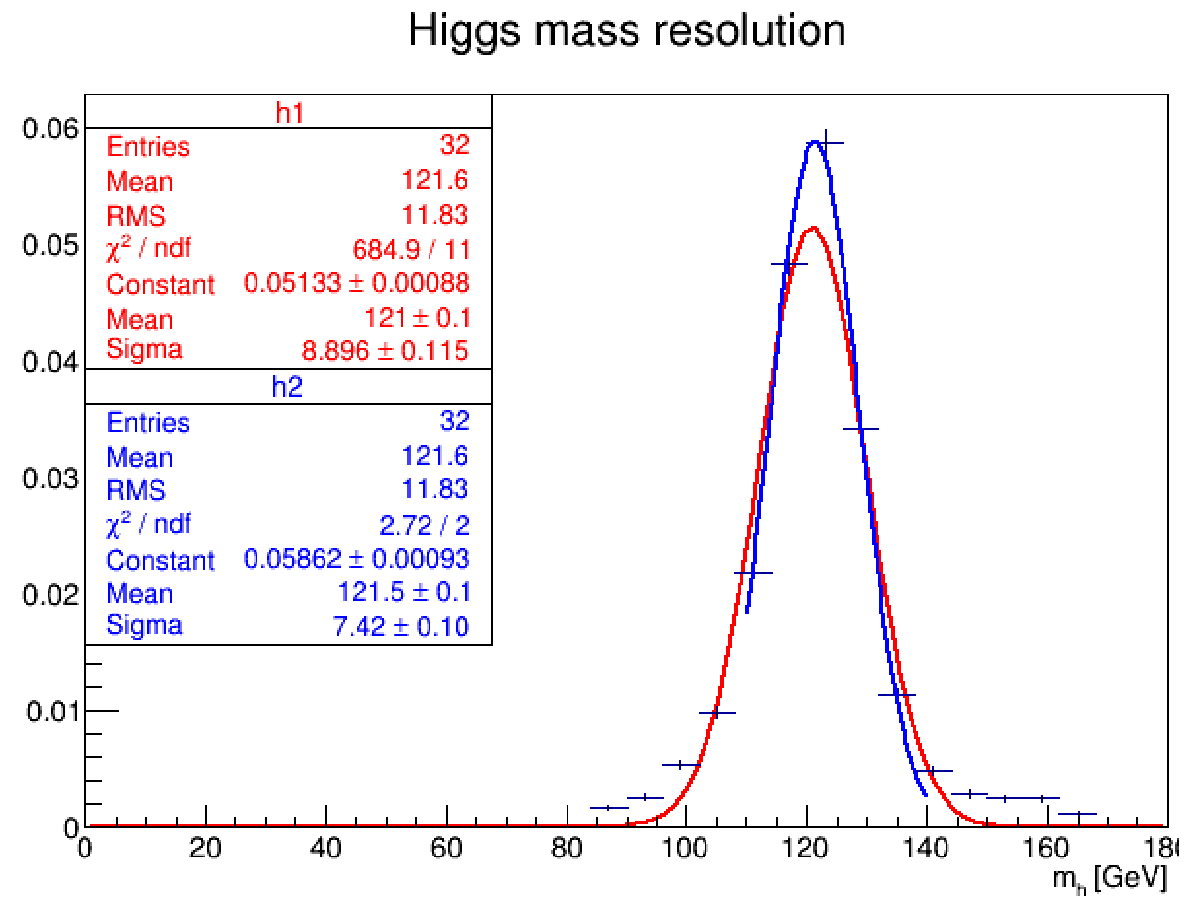
\includegraphics[width=0.49\textwidth]{plots/higgs_mass_res_noPU.pdf}
  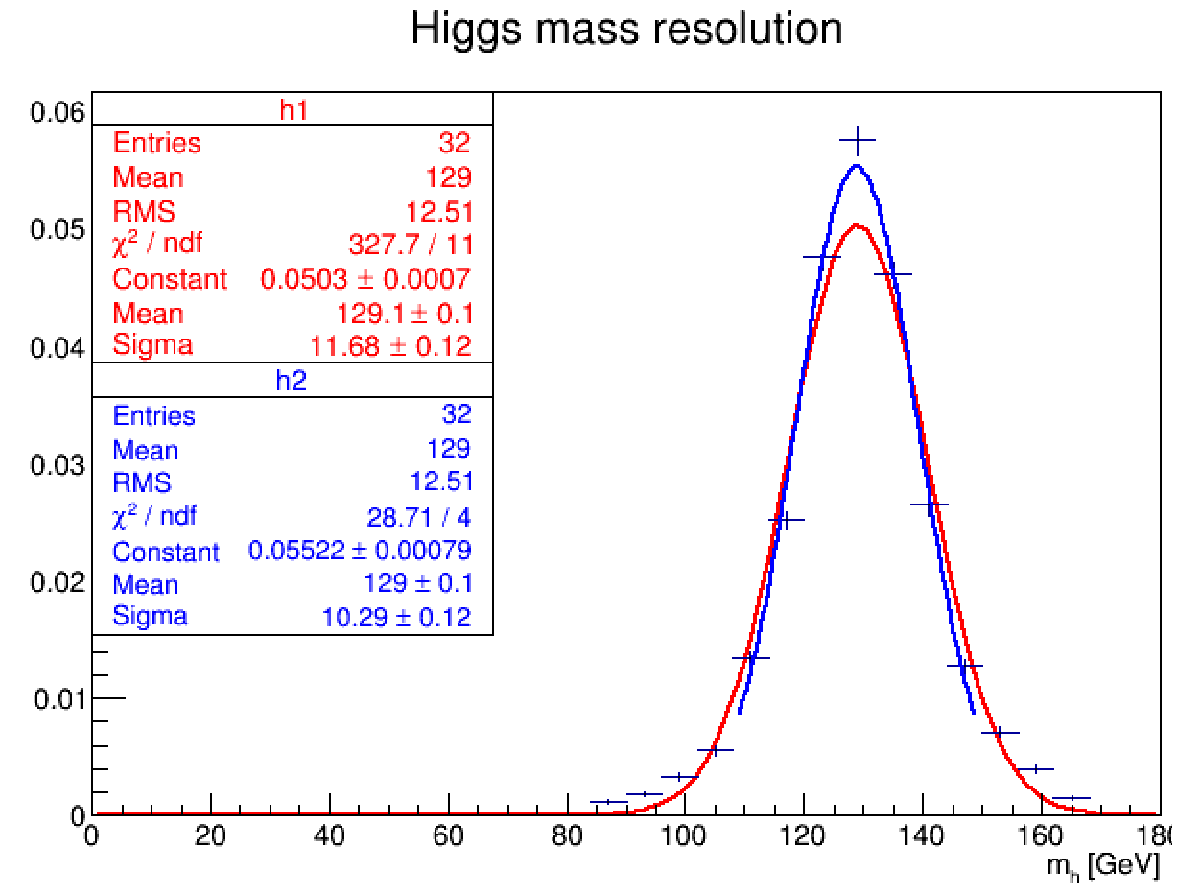
\includegraphics[width=0.49\textwidth]{plots/higgs_mass_res_PU80.pdf}
  \caption{\small The invariant mass distributions of the leading
    Higgs candidates in signal events for the resolved category, without
    PU (left plot) and with PU (right plot),
    together with Gaussian fits  used to determine the mass resolution.
    %
    In the latter case, $\la n_{\rm PU}\ra=80$, with {\tt SoftKiller}
     used for PU subtraction.
}
\label{fig:higgs-mass-resolution}
\end{center}
\end{figure}
%%%%%%%%%%%%%%%%%%%%%%%




%%%%%%%%%%%%%%%%%%%%%%%%%%%%%%%%%%%%%%%%%%%%%%%%%%%%
